
Почему мы вообще говорим о вычислении \textbf{g}-фактора заданного квантового состояния? Разве отношение механического и магнитного моментов не есть величина, постоянная для данного атома? Оказывается нет, и связано это с тем удивительным 
обстоятельством, что отношение магнитного $\vec{\mu}$ и механического $\vec{P}$ моментов электрона различно для орбитального и 
спинового моментов: 
\begin{gather} 
\label{eq:12} 
\mu_{L_i} = -\gamma \vec{P_{L_i}}, \\
\mu_{S} = -2\gamma \vec{P_{S_i}}, 
\end{gather}

$\gamma=\frac{e}{2mc}$ - \textbf{гиромагнитное отношение}.

Поскольку в различных квантовых состояниях орбитальные и спиновые моменты электронов дают различный вклад в величину механического момента атома $P_J$, соотношение между $\mu_H$ и $P_{J_H}$  в формуле (\ref{eq:7}), то есть \textbf{g}-фактор, оказывается также зависящим от квантового состояния. Для нахождения величины \textbf{g} следует, таким образом, найти среднюю по времени проекцию суммарного магнитного момента атома на направление внешнего магнитного поля $\vec{H}$ в данном квантовом состоянии.

Квантовомеханический расчет магнитных свойств многоэлектронных атомов представляет собой весьма сложную задачу, даже если пренебречь механическим и магнитным моментом ядра. В общем случае {\itshape{\textbf{кулоновское самосогласованное поле}}} в атоме является {\itshape\textbf{центрально-симметричным}} с точностью до так называемого {\itshape\textbf{остаточного} взаимодействия}, величина которого, как правило, существенно больше релятивистского взаимодействия спинового $\vec{P_{S_i}}$ и $\vec{P_{L_i}}$ моментов для каждого из электронов оболочки.

В некоторых тяжелых атомах и атомах, содержащих почти заполненные электронные оболочки, возможны случаи, когда {\itshape\textbf{спин-орбитальное}} взаимодействие превышает остаточное. В этих условиях пара моментов $\vec{P_{L_i}}$ и $\vec{P_{S_i}}$ электрона оболочки взаимодействует между собой сильнее, чем с моментами $\vec{P_{L_i}}$ и $\vec{P_{S_i}}$ других электронов. Поэтому образуются результирующие моменты $\vec{P_{j_i}}$ для каждого электрона в отдельности, которые затем уже объединяются в $\vec{P_J}$ атома. Такой вид связи носит название {\itshape\textbf{jj-связи}}.

Пренебрежение же спин-орбитальным взаимодействием по сравнению с остаточным носит название приближения {\itshape\textbf{[L-S]-}} (или {\itshape\textbf{нормальной}}, или {\itshape\textbf{Рассела-Саундерса}}) связи. Приближение {\itshape\textbf{[L-S]-}}-связи позволяет находить результирующие орбитальный
\begin{equation} 
\label{eq:14} 
\vec{\mu_L} = \sum_{i=1}^N \vec{\mu_{L_{i}}}=
-\gamma \sum_{i=1}^N\vec{P_{L_i}}=-\gamma \vec{P_L}
\end{equation}
и спиновый
\begin{gather} 
\label{eq:15} 
\vec{\mu_S} = \sum_{i=1}^N \vec{\mu_{S_{i}}}=-2\gamma \sum_{i=1}^N \vec{P_{S_i}}=-2\gamma \vec{P_S}
\end{gather}
магнитные моменты всей электронной оболочки (\textbf{N}- число электронов в оболочке) атома с помощью {\itshape\textbf{векторной}} модели. При этом полный магнитный момент атома
\begin{gather} 
\label{eq:16} 
\vec{\mu_J} =\vec{\mu_L}+\vec{\mu_S}=-\gamma(\vec{P_L}+2\vec{P_S})
\end{gather}
оказывается неколлинеарным его механическому моменту, что проиллюстрировано на рис. \ref{fig:2}.
\begin{gather} 
\label{eq:17} 
\vec{P_J}=\vec{P_L}+\vec{P_S},
\end{gather}

\begin{figure}[H]
    \centering
    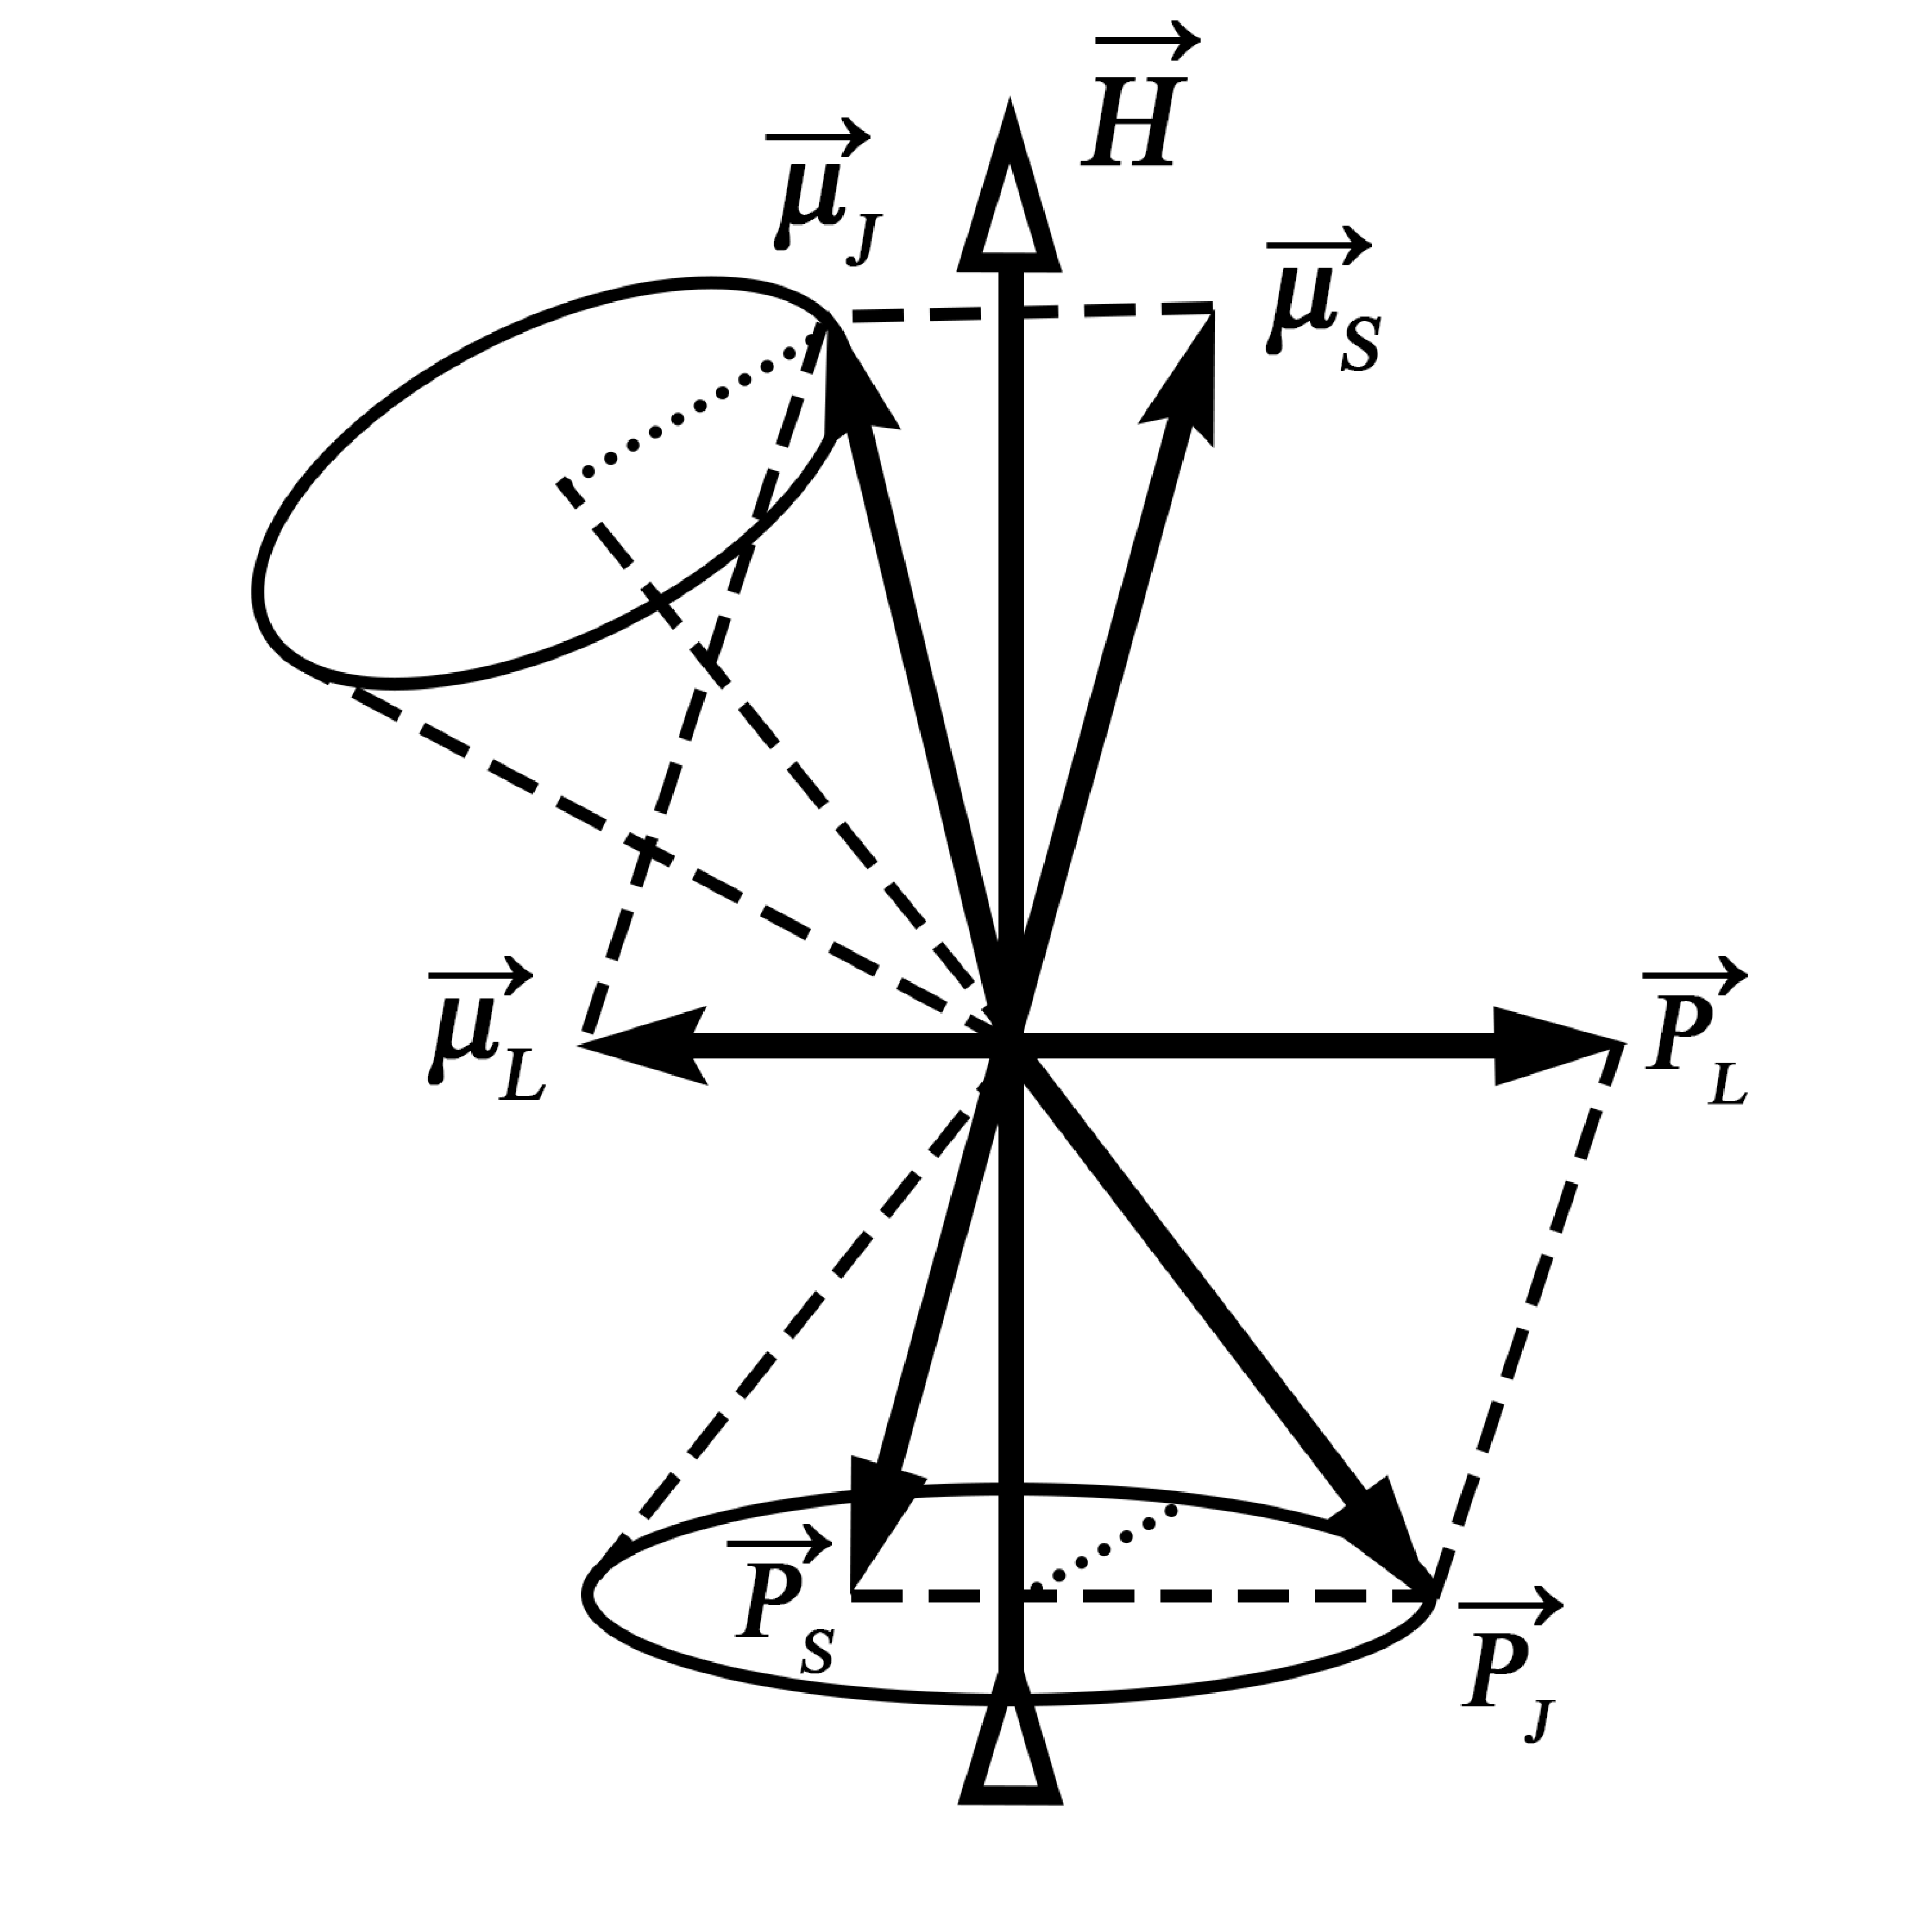
\includegraphics[width=.7\textwidth]{fig/fig2.pdf}
    \caption{Векторная модель атома}    
    \label{fig:2}
\end{figure}


Согласно правилам построения векторной модели складываемые результирующие моменты $\vec{P_L}$ и $\vec{P_S}$ (а вместе с ними и магнитные моменты $\vec{\mu_J}$,$\vec{\mu_L}$,$\vec{\mu_S}$ на векторной диаграмме рис. \ref{fig:2}) прецессируют вокруг направления результирующего момента $\vec{P_J}$. Скорость прецессии пропорциональна величине спин-орбитального взаимодействия.

Качественный вид зеемановского спектра оказывается различным в зависимости от соотношения между величинами взаимодействия результирующих моментов друг с другом и магнитным полем.

Рассмотрим два случая:

1)\textbf{сильное поле} - действие поля на каждый из моментов $\vec{P_L}$ и $\vec{P_S}$ превосходит взаимодействие их между собой

2)\textbf{слабое поле} - взаимодействие моментов друг с другом больше взаимодействия на каждый из них магнитного поля.

\textbf{1)} Внешнее магнитное поле $\vec{H}$ разрывает связь между результирующими моментами $\vec{P_L}$ и $\vec{P_S}$, и каждый из них прецессирует вокруг направления поля независимо другого. Проектироваться на направление поля $\vec{H}$ векторы $\vec{P_L}$ и $\vec{P_S}$ (а значит и векторы $\vec{\mu_L}$ и $\vec{\mu_S}$) будут тоже каждый в отдельности: $\vec{\mu_H}=-\gamma \hbar(M_L+2M_S)$, то есть расщепление оказывается целым кратным $\mu_0 H$. Для переходов имеют место правила отбора: $\Delta M_L=0,\pm 1; \Delta M_S=0.$ В результате получается триплет, совпадающий по виду с {\itshape\textbf{нормальным зеемановским триплетом}}, а само явление называется {\itshape\textbf{эффектом Пашена-Бака}}. Этот эффект наблюдается при $H\geq 2*10^5 \text{э}$, когда магнитное расщепление линий становится больше {\itshape\textbf{мультиплетного}} (связанного со спин-орбитальным взаимодействием) расщепления.

\textbf{2)} В случае {\itshape\textbf{слабого магнитного поля}} (именно этот случай реализуется в условиях нашего эксперимента) магнитный момент атома $\vec{\mu_J}$ прецессирует вокруг направления $\vec{H}$ (вместе с вектором $\vec{P_J}$), как это известно из классической механики, но и вокруг самого вектора $\vec{P_J}$. Поскольку частота {\itshape\textbf{классической (ларморовской)}} прецессии пропорциональна величине $H$, в достаточно слабых полях ларморовскую прецессию можно считать медленной по сравнению с прецессией вокруг $\vec{P_J}$. Усредняя $\vec{\mu_J}$ по периоду "быстрой" прецессии, находим, что средний по времени магнитный момент атома $\vec{\mu}$ совпадает с проекцией $\vec{\mu_J}$ на направление $\vec{P_J}$, то есть равен: 
\begin{gather} 
\label{eq:18} 
\mu=\mu_L \cos(\widehat{\vec{\mu_L},\vec{P_J}})+\mu_S \cos(\widehat{\vec{\mu_S},\vec{P_J}})
\end{gather}

Из элементарной геометрии Согласно рис.\ref{fig:21} следует:
\begin{equation} 
\label{eq:19a} 
\cos(\widehat{\vec{P_L},\vec{P_J}})=\frac{P_J^2+P_L^2-P_S^2}{2P_L P_J},
\end{equation}

\begin{gather} 
\label{eq:19b} 
\cos(\widehat{\vec{P_S},\vec{P_J}})=\frac{P_J^2+P_S^2-P_L^2}{2P_S P_J},
\end{gather}
что позволяет переписать равенство (\ref{eq:18}) в виде:
\begin{gather} 
\label{eq:20} 
\mu=\gamma P_J(1+\frac{P_J^2+P_S^2-P_L^2}{2P_J^2}=\mu_0 \text{g} \frac{P_J}{\hbar}.
\end{gather}
 
 Подстановка формул вида (\ref{eq:6}) в (\ref{eq:20}) позволяет сразу найти связь между механическим $P_J$ м "эффективным" магнитным моментом атома $\mu$ в состоянии с квантовыми числами \textbf{J, L, S}, то есть \textbf{g}-фактор данного квантового состояния:
\begin{gather} 
\label{eq:21} 
\text{g}=1+\frac{J(J+1)+S(S+1)-L(L+1)}{2J(J+1)}
\end{gather}